\thispagestyle{quantoannone}
\pagestyle{quantoan}
\everymath{\color{quantoan}}
\graphicspath{{../quantoan/pic2/}}
\blfootnote{\color{quantoan}\color{quantoan}$^*$Nguồn Math. Intellegencer, Số $41$.}
\begingroup
\AddToShipoutPicture*{\put(0,616){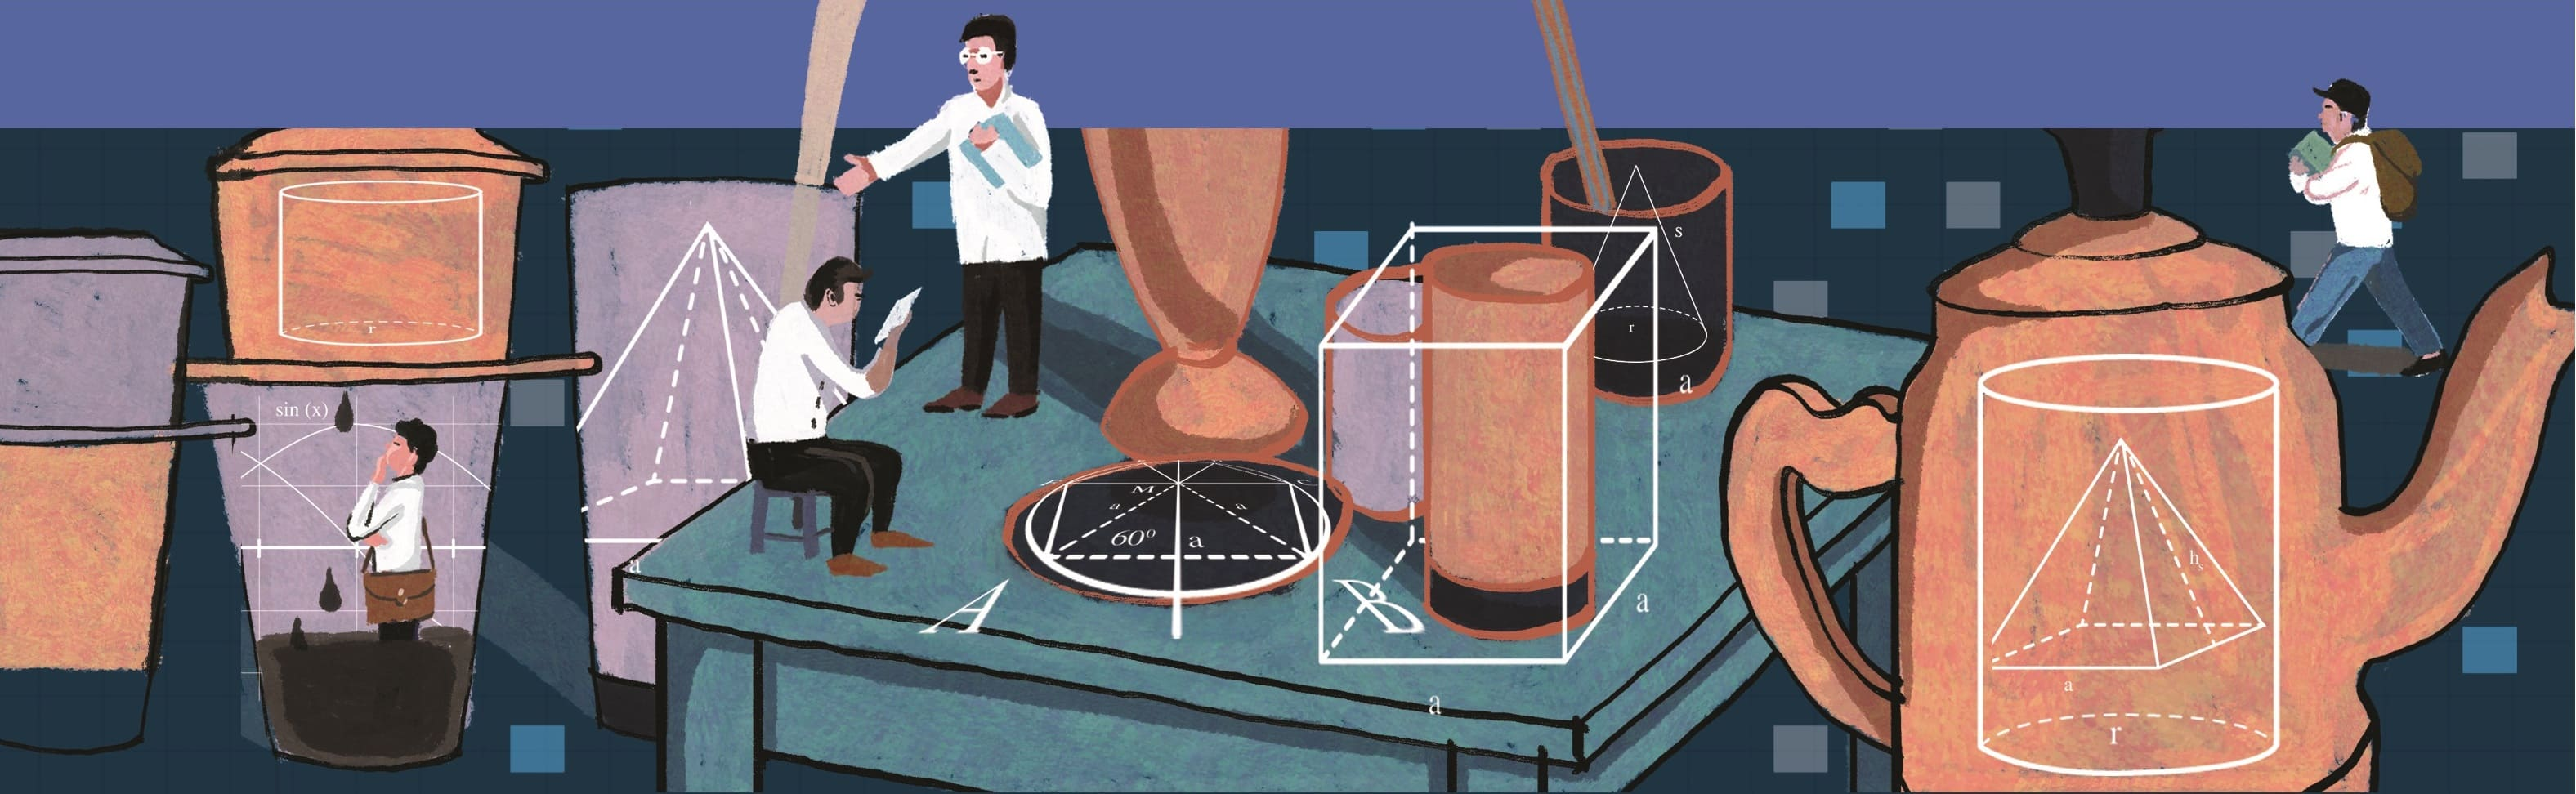
\includegraphics[width=19.3cm]{../bannerquantoan}}}
\AddToShipoutPicture*{\put(58,505){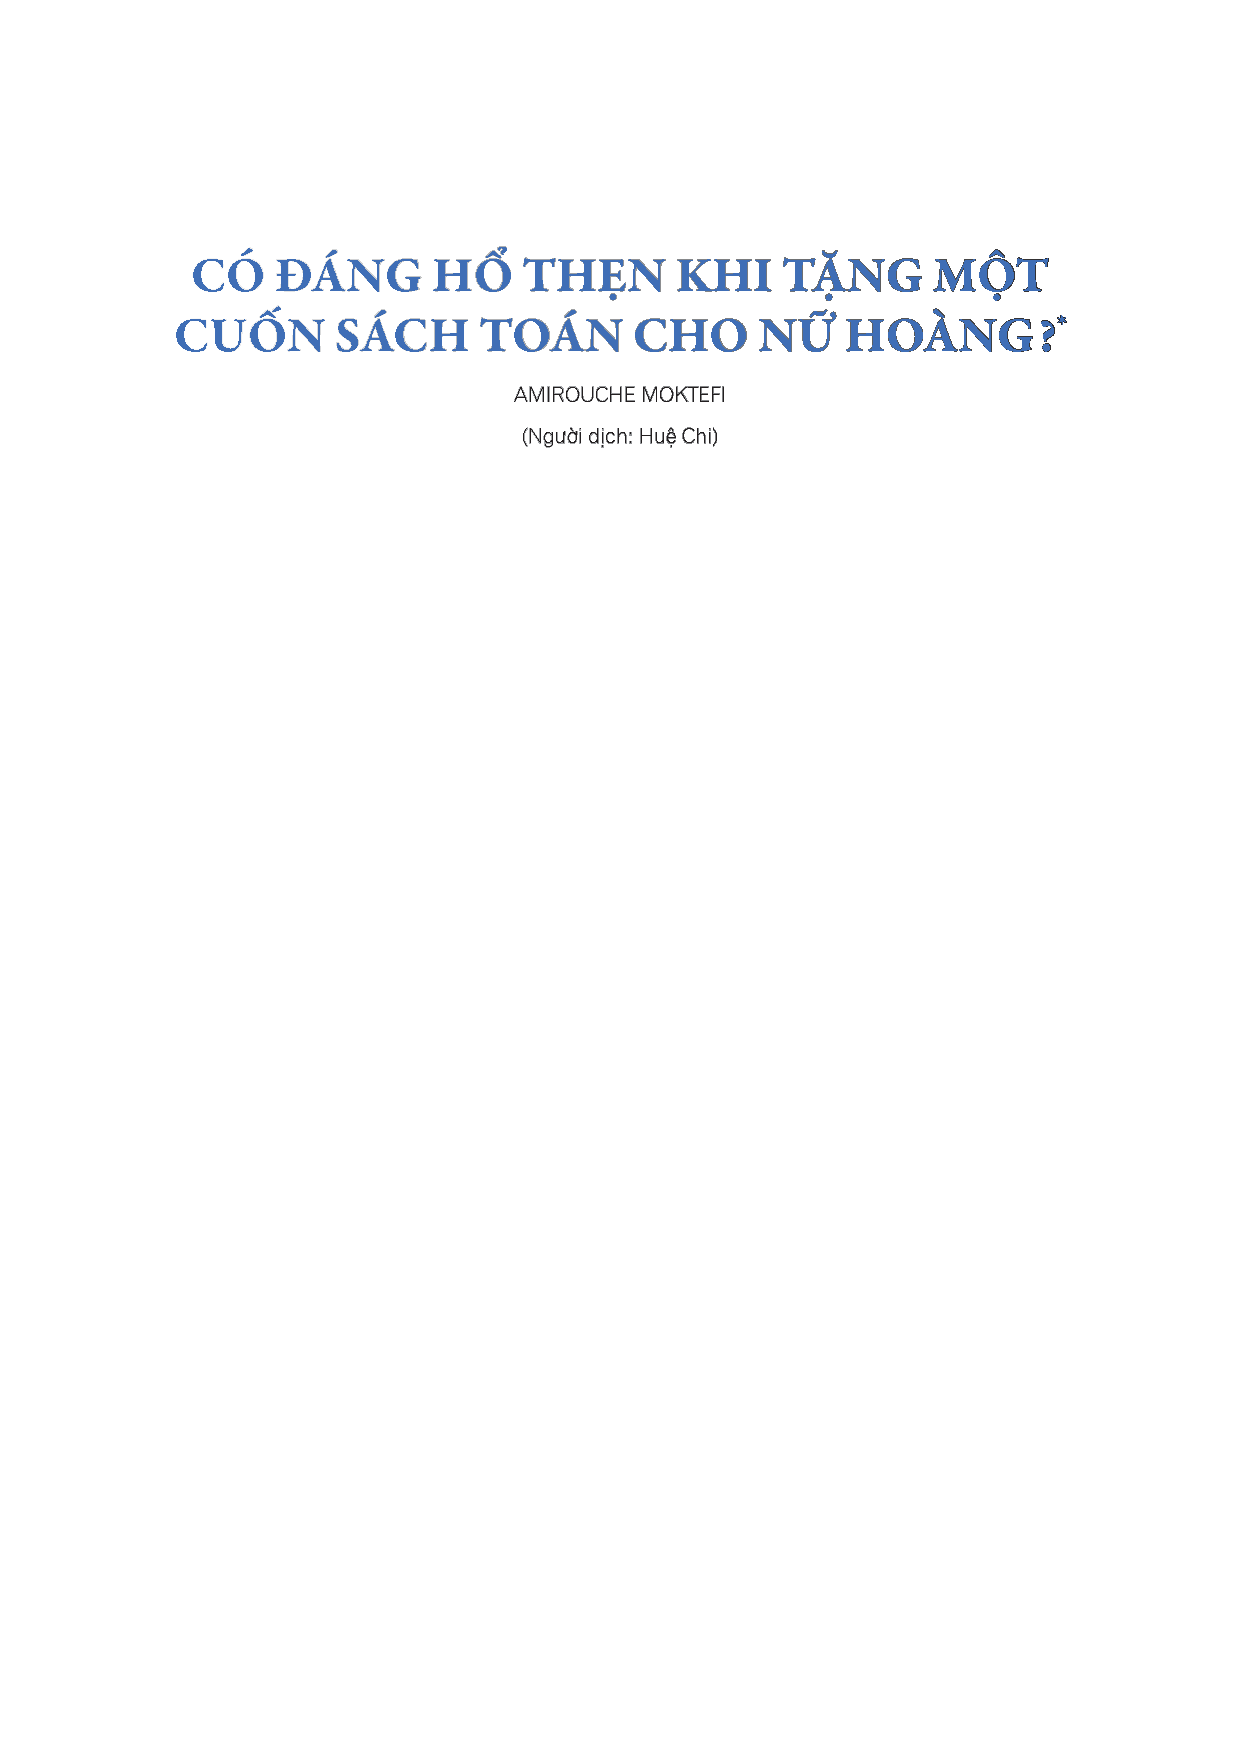
\includegraphics[scale=1]{../tieude.pdf}}}
\centering
\endgroup

\vspace*{198pt}

\begin{multicols}{2}
	Ai cũng biết rằng Charles Lutwidge Dodgson (bút danh Lewis Carroll, $1832-1898$; Hình $1$), tác giả của \textit{Alice ở xứ xở diệu kỳ}, là một nhà toán học. Dodgson là một giảng viên toán tại trường Christ Church thuộc Đại học Oxford và đã có nhiều công trình toán học về hình học, đại số, logic và lý thuyết bỏ phiếu. Hầu hết mọi đánh giá về toán học của Dodgson đều nhắc đến một câu chuyện thú vị (sau đây gọi là \textit{câu chuyện}) liên quan đến nữ hoàng Victoria. Nữ hoàng được cho là rất thích truyện \textit{Alice}, xuất bản năm $1865$, và đã yêu cầu tác phẩm tiếp theo của tác giả. Với sự ngạc nhiên và thất vọng, bà đã nhận được cuốn \textit{Chuyên luận về định thức} của Dodgson, xuất bản năm $1867$. Câu chuyện này là một giai thoại kinh điển mà người ta thường bắt gặp trong các tác phẩm về toán học.
	\vskip 0.02cm
	Những bài viết về \textit{câu chuyện} cũng đôi khi nhắc nhở chúng ta rằng chính Dodgson đã phủ nhận nó vào năm $1896$, nhưng sự lan rộng của tin đồn dường như không thể ngăn được. Có thể dễ dàng hiểu được sức hấp dẫn của nó, vì nó thể hiện một cách hoàn hảo quan niệm rộng rãi về Dodgson nói riêng và toán học nói chung. Đầu tiên, câu chuyện truyền tải một cái nhìn rộng rãi về Dodgson như một nhân vật kép: một mặt là nhà toán học buồn tẻ và mặt khác là một tiểu thuyết gia giàu trí tưởng tượng. Thứ hai, phản ứng được cho là của nữ hoàng tiêu biểu cho niềm tin rằng toán học và văn học bắt nguồn từ những bộ óc và nền văn hóa khác nhau. Điều thú vị là nhiều lời kể về \textit{câu chuyện} nói rằng nữ hoàng không hài lòng khi nhận được cuốn sách. Người ta cũng nói rằng Dodgson, người rất tôn kính hoàng gia, không thể nào thực hiện một ``hành động hoàn toàn ngược với tính cách" như vậy (Beale $1973$). Nhưng  tặng một cuốn sách toán cho nữ hoàng thì có gì sai?  
	\begin{figure}[H]
		\vspace*{-5pt}
		\centering
		\captionsetup{labelformat= empty, justification=centering}
		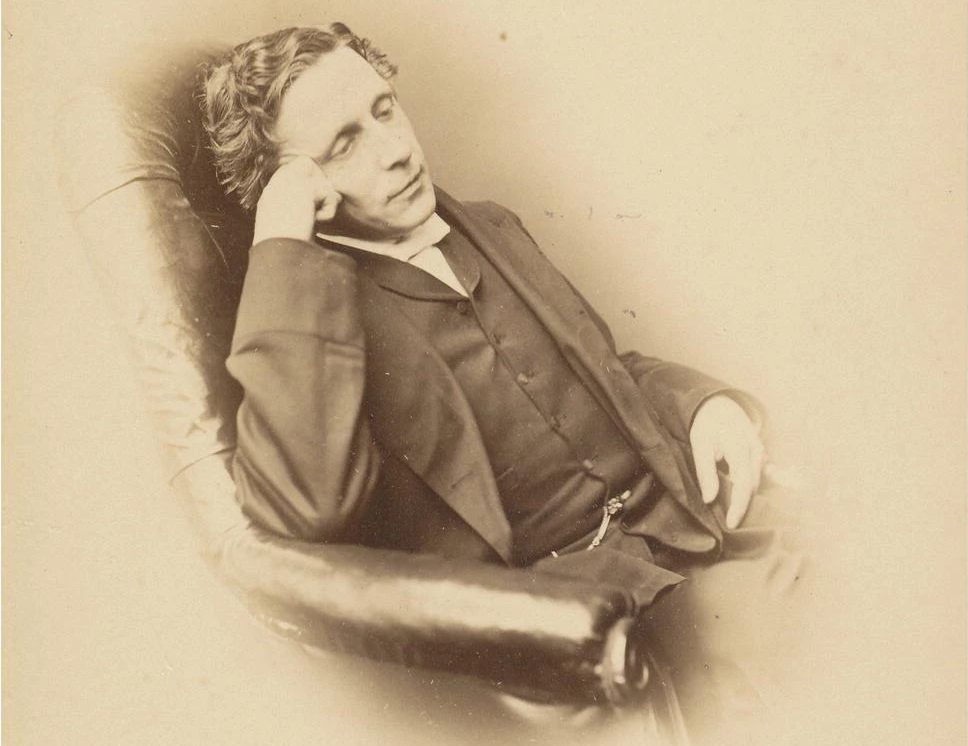
\includegraphics[width= 1\linewidth]{1}
		\caption{\small\textit{\color{quantoan}Hình $1$. Charles L. Dodgson (from the Wakeling
				Collection).}}
		\vspace*{-5pt}
	\end{figure}
	\textbf{\color{quantoan}Câu chuyện lan truyền chóng mặt}
	\vskip 0.1cm
	Khi \textit{Alice ở xứ xở diệu kỳ} ra mắt (Dodgson $1865$, Hình $2$), Dodgson là một tác giả vô danh. Ông mới chỉ xuất bản một số tập sách nhỏ về toán học và các tác phẩm nhỏ. Đặc biệt, vào năm $1856$, ông đã đóng góp một số bài thơ cho tạp chí \textit{Chuyến tàu}, ở đó ông sử dụng bút danh Lewis Carroll, lấy từ tên của mình (Lewis từ Lutwidge và Carroll từ Charles). Những năm sau đó, ông chủ yếu sử dụng tên thật cho các công trình toán học và bút danh cho các tác phẩm văn học để giữ kín danh tính của mình. Thành công tức thì của cuốn sách \textit{Alice} đã làm cho bút danh văn học của ông được đông đảo công chúng biết đến, nhưng họ không biết được ông có thể là ai.
	\begin{figure}[H]
		\vspace*{-5pt}
		\centering
		\captionsetup{labelformat= empty, justification=centering}
		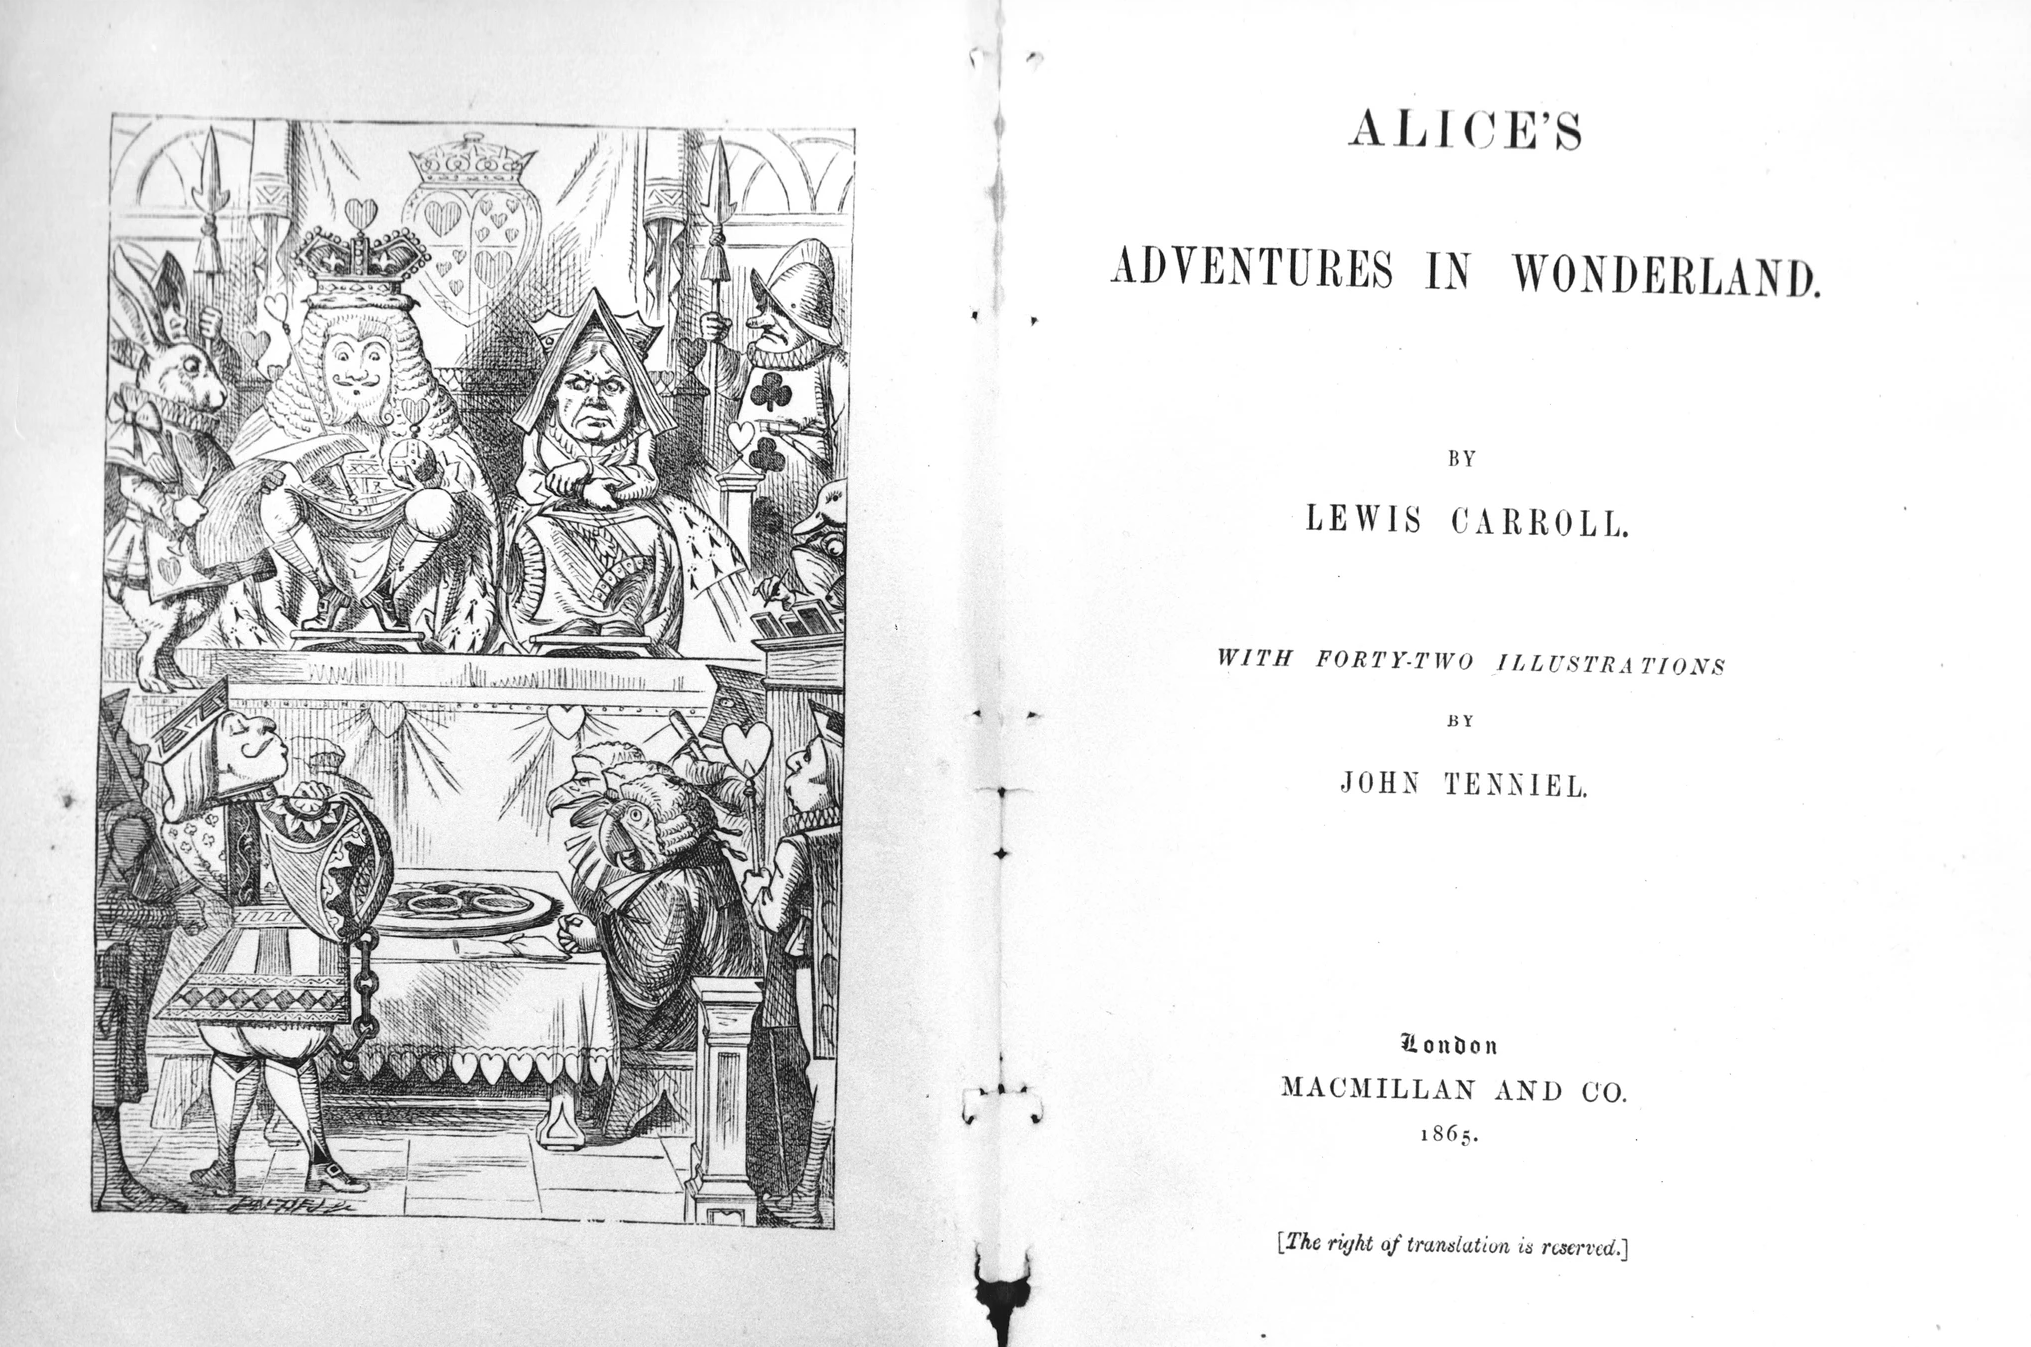
\includegraphics[width= 1\linewidth]{2}
		\caption{\small\textit{\color{quantoan}Hình $2$. The title page of Dodgson’s Alice’s Adventures in Wonderland, $1865$ (Photo by George Bayntun, Collection of Charlie Lovett).}}
		\vspace*{-10pt}
	\end{figure}
	Cuốn sách cũng được hưởng một nỗ lực quảng bá lớn của cả nhà xuất bản và tác giả. Vô số các bản sao đã được gửi đến các tạp chí để đánh giá, hoặc tặng bạn bè làm quà. Cháu trai, đồng thời là người viết tiểu sử đầu tiên của Dodgson, Stuart D. Collingwood, đã thuật lại rằng bản sao đầu tiên của cuốn sách được gửi đến Alice ngoài đời thực, người đã truyền cảm hứng cho câu chuyện, còn bản thứ hai được gửi đến công chúa Beatrice, con gái út của nữ hoàng Victoria (Collingwood $1898$, tr.$104$) . Đáp lại, Dodgson nhận được một lá thư cho biết ``cuốn sách nhỏ mà Bệ hạ rất hài lòng khi cho phép đọc nó cho công chúa Beatrice" (Wakeling $1999$, tr. $122$).
	\vskip 0.1cm
	Với sự khen ngợi của giới phê bình và số lượng lớn sách bán được, ý tưởng về phần tiếp theo hẳn đã nhanh chóng nảy ra với Dodgson và nhà xuất bản của ông. Ngay từ năm $1866$, Dodgson đã đề cập đến việc ``đang cân nhắc ý tưởng về việc viết một thứ kiểu như phần tiếp theo". Công chúng rõ ràng đã mơ màng về những cuộc phiêu lưu khác, và có tin đồn rằng ``Lewis Carroll đang viết tiếp" (Collingwood $1898$, tr.$129$).
	\vskip 0.1cm
	Quả thực là Dodgson đang viết. Bên cạnh những thứ khác, ông đang nghiên cứu về thứ có thể là đóng góp quan trọng nhất của ông cho nghiên cứu toán học. Thật vậy, ông đã đưa ra một phương pháp mới để tính toán các định thức, trình bày nó trước Hiệp hội Hoàng gia Luân Đôn vào tháng $5$ năm $1866$, và sau đó công trình này xuất hiện trong Kỷ yếu của Hiệp hội Hoàng gia Luân Đôn. Trong vòng một năm sau đó, Dodgson đã phát triển bài báo của mình thành một ``cuốn sách nhỏ", mà ông ghi lại trong nhật ký của mình là ``đã mang lại cho [ông] nhiều rắc rối hơn bất cứ thứ gì mà ông đã từng viết" (Wakeling $1999$, $206-207$). Việc xuất bản cuốn sách bị gián đoạn bởi một chuyến đi đến nước Nga cùng với Henry Parry Liddon từ tháng $7$ đến tháng $9$ năm $1867$. \textit{Chuyên luận về định thức} cuối cùng được xuất bản vào đầu tháng $12$ năm đó (Hình $3$). Cuốn sách này đã nhận được một số lời khen ngợi về đóng góp và tính mới, nhưng bị chỉ trích vì văn phong logic nặng nề và sự lựa chọn thuật ngữ và ký hiệu gây khó đọc.
	\vskip 0.1cm
	\textit{Chuyên luận về định thức} là cuốn sách đầu tiên của Dodgson kể từ Alice, nhưng nó không có liên hệ gì với cuốn truyện tuyệt vời đó. Trước khi hoàn thành, Dodgson đã thông báo cho nhà xuất bản của mình, Macmillan, trong một bức thư ngày $11$ tháng $2$ năm $1867$, về ý định đề tên thật của mình cho cuốn sách: ``Tôi có một cuốn sách nhỏ, sắp hoàn thành, mà tôi muốn các ông xuất bản cho tôi -- nhưng tôi e rằng nó không thể được giới thiệu như là của tác giả 'của \textit{Những cuộc phiêu lưu của Alice}'". Độc giả của chuyên luận chắc chắn không có lý do gì để nghi ngờ rằng tác giả của nó thực sự là người đã viết ra \textit{Alice}. Vào thời điểm đó, Dodgson đã giữ được bí mật danh tính của mình và chỉ tiết lộ nó cho một số bạn bè và những người quen may mắn. Những bức thư gửi cho Lewis Carroll được gửi đến nhà xuất bản Macmillan, sau đó nhà xuất bản chuyển tiếp tới ông dưới cái tên Charles L. Dodgson ở Oxford. Khi một cô bé yêu cầu ông viết một câu chuyện Alice khác vào năm $1867$, ông hồi âm dưới cái tên Dodgson, khẳng định rằng ông có một thông điệp cho cô ấy ``từ một người bạn ... ông Lewis Carroll, một sinh vật kỳ dị, khá thích nói những chuyện vô nghĩa".
	\begin{figure}[H]
		\vspace*{-5pt}
		\centering
		\captionsetup{labelformat= empty, justification=centering}
		
\includegraphics[width= 1\linewidth]{3}
		\caption{\small\textit{\color{quantoan}Hình $3$. The title page of Dodgson’s Elementary Treatise on Determinants, $1867$ (from the Wakeling Collection)}}
		\vspace*{-10pt}
	\end{figure}
	Khi \textit{Chuyên luận về định thức} ra mắt, có lẽ chỉ có một nhóm nhỏ độc giả có đặc quyền mới biết được bí mật nhỏ của tác giả, và ``nó là một phát hiện hoàn toàn bất ngờ với những sinh viên đại học lần đầu tiên được biết rằng ông Dodgson của trường Christ Church và Lewis Carroll chính là một" (Colingwood $1898$, tr.$110$). Một trong những người viết đánh giá về chuyên luận dường như biết điều đó, vì ông ta kết thúc bài đánh giá của mình bằng cách hy vọng ``có thêm khảo sát về thế giới thần tiên đại số tùy chọn [của tác giả]". Sự ám chỉ này đến truyện \textit{Alice} chắc hẳn đã khiến Dodgson khó chịu, một người đã rất cố gắng giữ bí mật về danh tính của mình. Dodgson phàn nàn trong một bức thư gửi cho chị dâu của mình, vào ngày $31$ tháng $7$ năm $1890$, rằng ông thấy khá kỳ lạ rằng ``mọi người sẽ không hiểu rằng, khi một tác giả sử dụng \textit{bút danh}, thì mục đích là \textit{tránh} việc công khai danh tính cá nhân, điều mà họ luôn cố gắng thúc giục anh ta". Có vẻ như việc Dodgson nhất quyết giữ bí mật danh tính của mình chỉ khiến những ``kẻ săn đuổi" ông trở nên đông đảo và quyết tâm hơn. Quả là tình huống đó hẳn đã gợi nên sự tò mò và hấp dẫn, và dễ dàng hình dung được sự ngạc nhiên của một độc giả nhiệt tình của \textit{Alice}, không biết rằng tác giả của nó là một giảng viên toán tại Oxford, khi đối diện với cuốn sách tiếp theo của tác giả, về chủ đề định thức, và được cho biết tác giả thực sự là ai. Những gì đã có thể là một giai thoại thú vị đã trở thành một câu chuyện lan truyền chóng mặt khi độc giả bối rối tình cờ lại chính là nữ hoàng.
	\vskip 0.1cm
	Câu chuyện này quá hay và không khó để có thể là sự thật. Thực sự là nữ hoàng biết, và có thể rất thích truyện \textit{Alice}. Bà  chỉ cần hỏi, và có thể bà ấy đã hỏi, về cuốn sách tiếp theo của tác giả, để khiến cho \textit{câu chuyện} xảy ra. Đó là một \textit{câu chuyện} tuyệt vời, và sẽ còn tuyệt vời hơn nếu Dodgson không hoàn toàn phủ nhận nó, gần ba mươi năm sau thời điểm mà nó được cho là đã xảy ra.
	\vskip 0.1cm
	\textbf{\color{quantoan}Phủ nhận} 
	\vskip 0.1cm
	Đến năm $1896$, Dodgson là một tác giả nổi tiếng từ chối tận hưởng danh tiếng của mình. Phần tiếp theo của câu chuyện, \textit{Đi qua tấm gương}, cũng  thành công như truyện \textit{Alice ở xứ sở diệu kỳ}.
	\vskip 0.1cm
	Sau đó, ông xuất bản nhiều tác phẩm hư cấu khác, nhưng không có tác phẩm nào thực sự sánh được với hai truyện \textit{Alice}. Là một nhà toán học, ông cũng đã xuất bản nhiều về nhiều chủ đề khác nhau, đặc biệt là bảo vệ một cách đẹp đẽ hình học Euclid trước những sách giáo khoa mới muốn thay thế nó trong các trường trung học và đại học. Trong những năm cuối đời, ông viết một chuyên luận về logic nhằm giúp chủ đề này có thể tiếp cận tới một công chúng rộng rãi. Không giống như các đồng nghiệp của mình tại Đại học Oxford, Dodgson đã chấp nhận lý thuyết logic hình thức mới được phát triển ở Anh bởi George Boole và những người theo trường phái của ông. Phần đầu tiên của chuyên luận của Dodgson, \textit{Logic hình thức}, xuất bản vào tháng $2$ năm $1896$. Lần tái bản thứ nhất, ra mắt vào đầu tháng $6$ cùng năm, có lời tựa được đề ngày $11$ tháng $5$ năm $1896$ (Hình $4$). Ngoài một vài thay đổi và sửa chữa nhỏ, nó có một phần tái bút sau trang tiêu đề, với ghi chú sau:
	\vskip 0.1cm
	\textit{Tôi xin nhân cơ hội này để phủ nhận một cách công khai nhất  có thể  một câu chuyện ngớ ngẩn, được lan truyền trên báo chí, về việc tôi đã tặng một số cuốn sách nào đó cho Nữ hoàng. Nó được lặp đi lặp lại liên tục, và là thêu dệt hoàn toàn, đến nỗi tôi nghĩ rằng đáng để tuyên bố, một lần dứt điểm, rằng nó tuyệt đối sai trong mọi chi tiết: không có bất kỳ điều gì thậm chí hơi giống như thế đã từng xảy ra cả.}
	\vskip 0.1cm
	Dodgson đã giữ ghi chú này trong lần tái bản thứ hai của cuốn sách, có lời tựa đề ngày $20$ tháng $7$ năm $1896$, nhưng vì lý do nào đó đã bỏ nó khỏi lần tái bản thứ ba, xuất bản vào đầu năm $1897$ nhưng có lời tựa vào Giáng sinh năm $1896$.
	\vskip 0.1cm
	Trong ghi chú này, Dodgson đã mạnh mẽ phủ nhận một ``câu chuyện ngớ ngẩn" về việc ông đã tặng một số cuốn sách cho nữ hoàng. Có thể lưu ý rằng giải thích của Dodgson là rất ít ỏi và có thể đề cập đến một sự việc khác, nhưng có vẻ như chỉ đơn giản là ông không muốn kể chi tiết về giai thoại để không quảng bá thêm về nó. Dodgson rõ ràng không thấy thích thú gì với \textit{câu chuyện}. Vì tin đồn đề cập đến các sự kiện được cho là diễn ra vào năm $1867$, một số tác giả tự hỏi tại sao Dodgson phải mất gần ba mươi năm để phủ nhận nó (Wakeling $2015$, tr. $315$). Derek Hudson cho rằng Dodgson có thể đã dùng thời gian này để tranh luận ``với chính bản thân mình liệu có đúng khi phản bác câu chuyện hay không (Hudson $1976$,  tr.$133$). Một lời giải thích hợp lý hơn có thể là Dodgson chỉ đơn giản là phủ nhận câu chuyện khi nó được lan truyền rộng ra, vì không có lý do gì để cho rằng tin đồn được bắt đầu trong cùng thời kỳ mà những sự việc được kể lại trong \textit{câu chuyện} được cho là đã xảy ra.
	\begin{figure}[H]
		\vspace*{-5pt}
		\centering
		\captionsetup{labelformat= empty, justification=centering}
		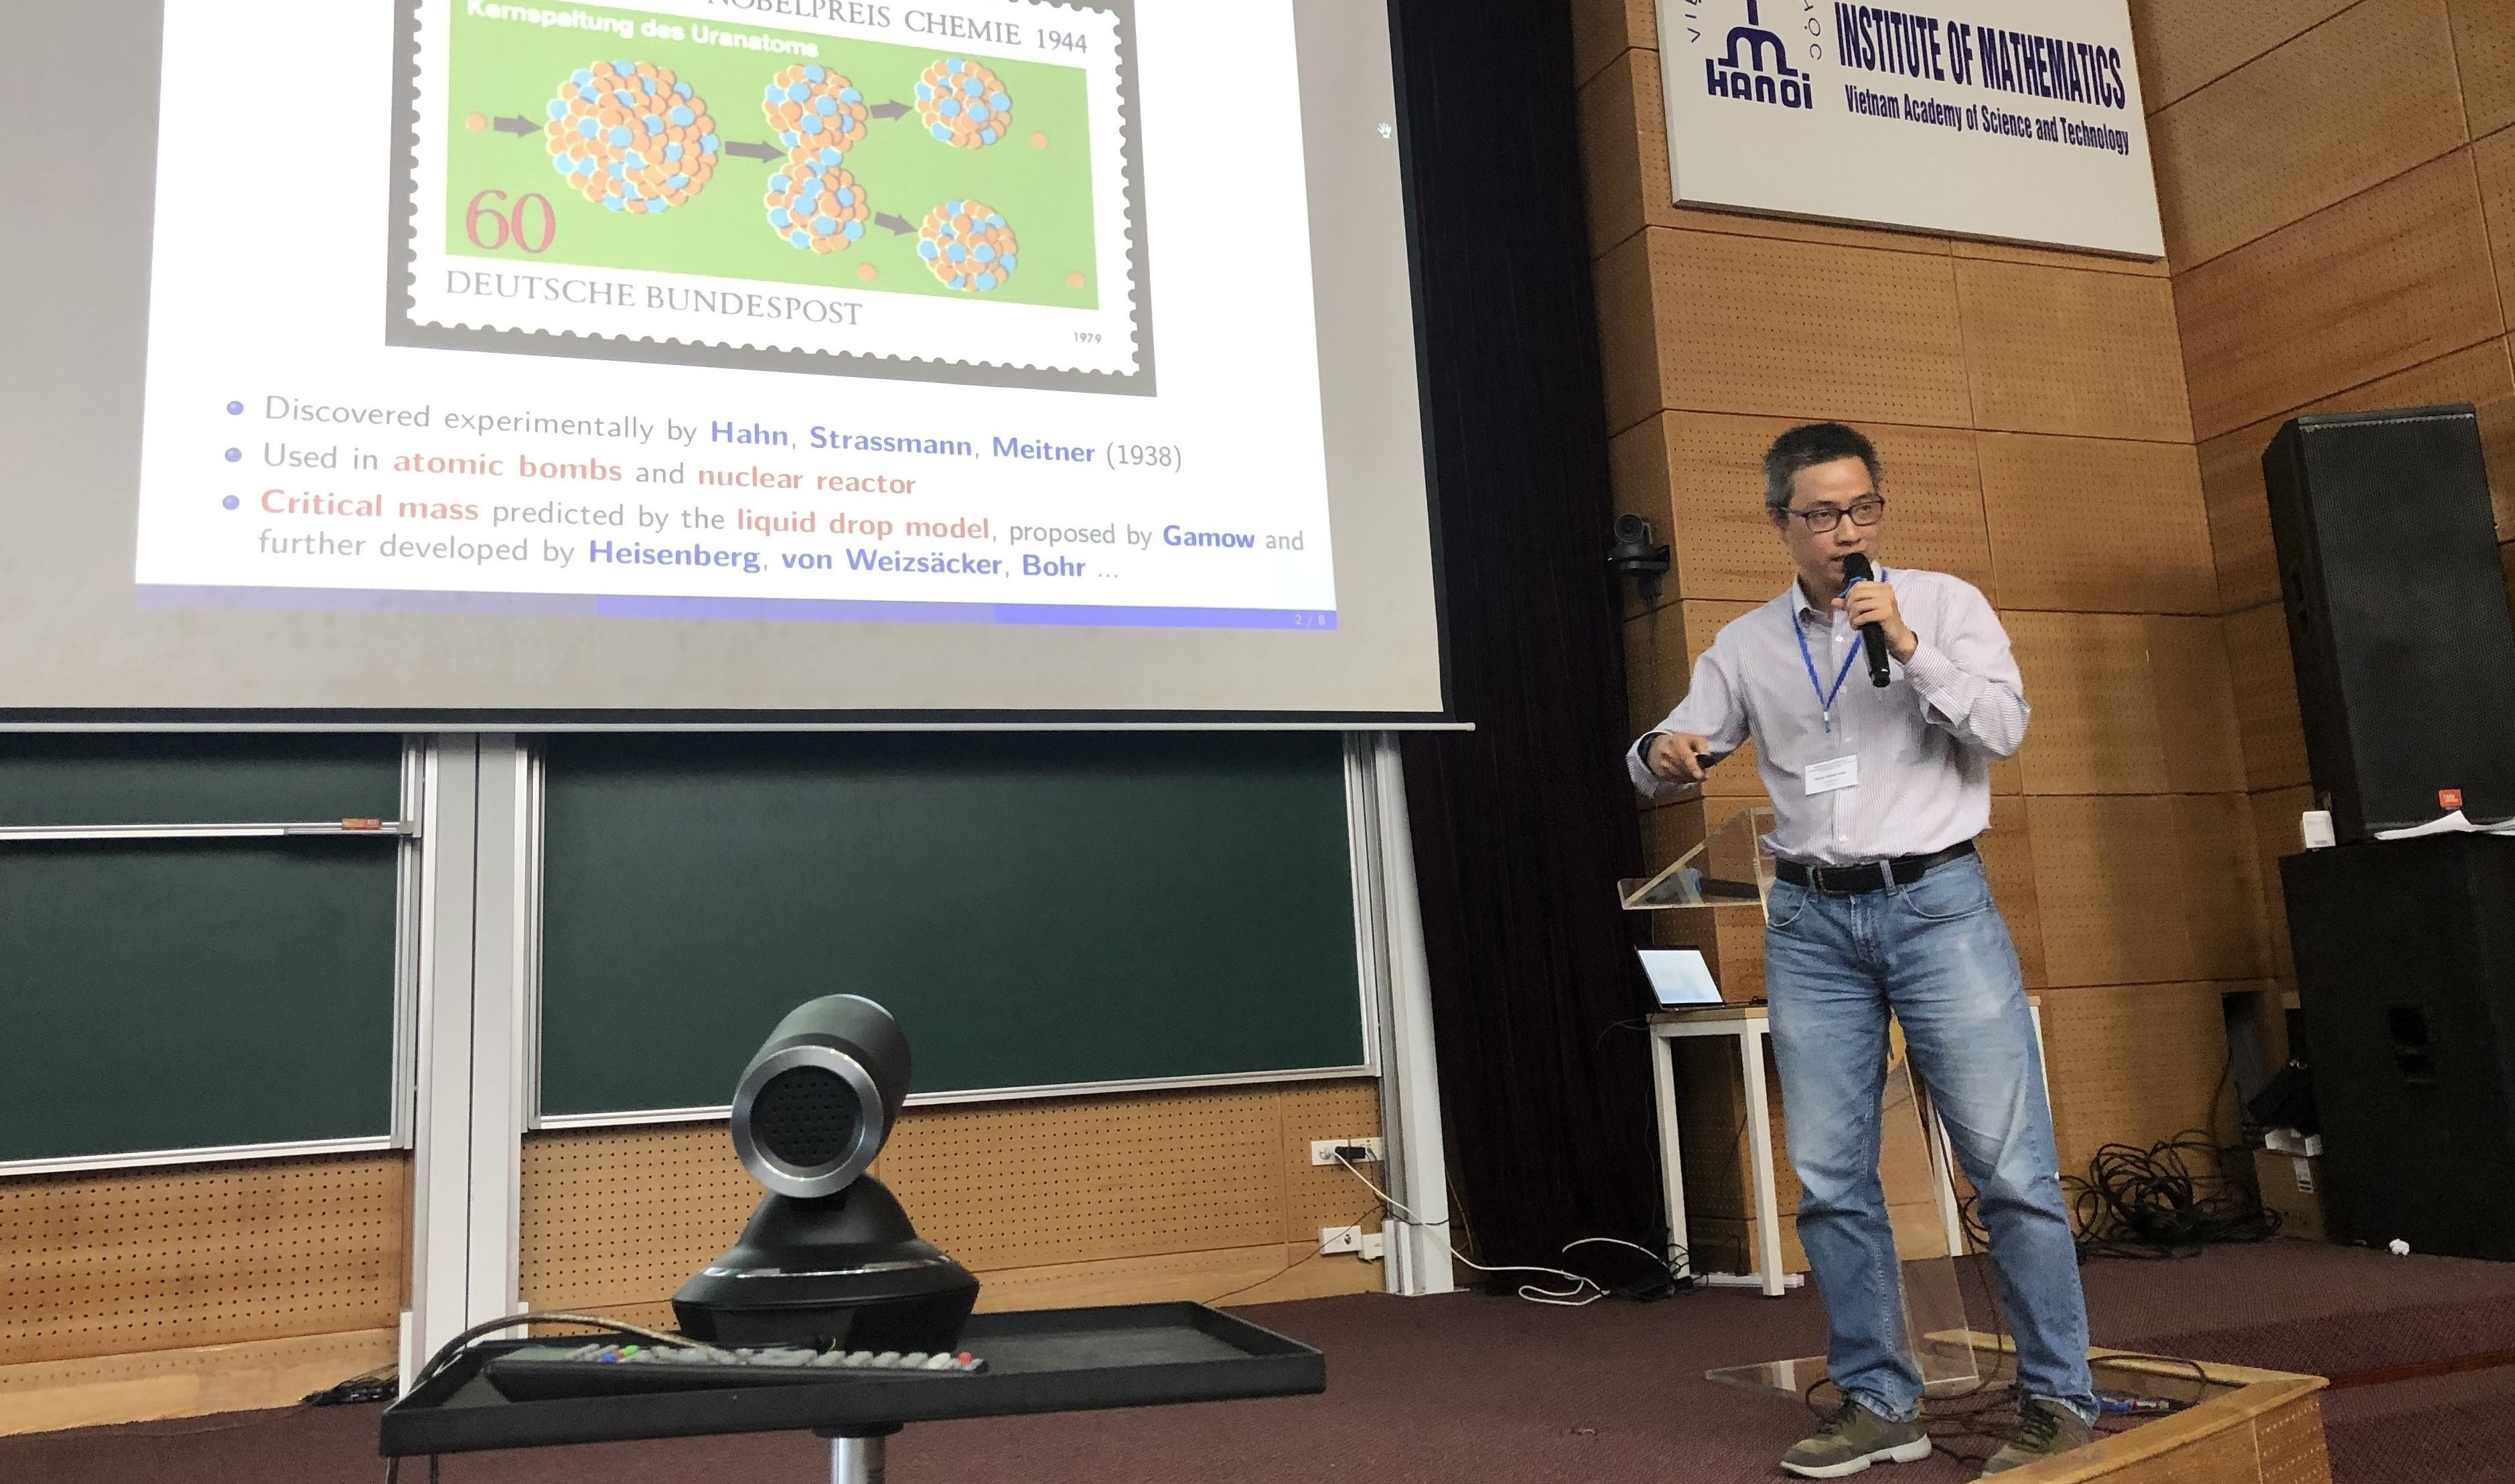
\includegraphics[width= 1\linewidth]{4}
		\caption{\small\textit{\color{quantoan}Hình $4$. The title page of Dodgson’s Symbolic Logic, second edition, $1896$, and the Advertisement page, which includes a denial of the story (from the Wakeling Collection).}}
		\vspace*{-10pt}
	\end{figure}
	Trên thực tế, có vẻ như không biết tin đồn đã bắt đầu từ khi nào. Trong một thời gian dài, người ta thậm chí đã nghĩ rằng không có bằng chứng văn bản nào về sự tồn tại của tin đồn trước sự phủ nhận của chính Dodgson vào năm $1896$. Tuy nhiên, trong những năm gần đây, một số bài báo trước đó về nó đã được tìm thấy, và giờ đây mọi thứ trở nên rõ ràng rằng tin đồn đã lan truyền khá rộng vào quãng thời gian mà Dodgson phủ nhận nó. Tin đồn chắc chắn tồn tại ít nhất từ năm $1892$, vì nó được tìm thấy trên một số tờ báo thời đó, chẳng hạn như \textit{Sporting Times}. Nó dường như đã được lan truyền rộng rãi hơn sau năm $1895$, đặc biệt là sau khi nó được Ethel Mackenzie McKenna kể lại trong số tháng $8$ năm $1895$ của \textit{Tạp chí Ladies’ Home}:
	\vskip 0.1cm
	``Trong thời kỳ  mới mẻ của sự thành công rực rỡ, ``Alice" nằm  trên tay của mọi người và những chuyến phiêu lưu vào thế giới thần tiên của cô là niềm vui thích của  người lớn cũng như trẻ em. Nữ hoàng Victoria đã gửi một thông điệp đến tác giả, xin ông gửi cho bà cuốn sách tiếp theo của mình. Giống như tất cả các thần dân của mình, bà nóng lòng muốn nghe nhiều hơn về đứa trẻ thú vị, mà nguyên mẫu là con gái của hiệu trưởng của trường Christ Church. Bà đã rất kinh ngạc khi không lâu sau đó nhận được một cuốn ``\textit{Chuyên luận về định thức}" của C. L. Dodgson, vì khi đó, ông vẫn giữ bí mật về danh tính của mình, và Nữ hoàng, cũng như cả thế giới, đã tin rằng ông chỉ đơn thuần là một người hài hước."
	\vskip 0.1cm
	Tạp chí của Mỹ này có lượng độc giả rộng lớn và ngày càng tăng vào thời Dodgson, và vào năm $1904$, nó trở thành tạp chí đầu tiên đạt được số lượng một triệu người đặt báo. Lời kể của McKenna về \textit{câu chuyện} được đăng lại trên các tạp chí khác của Mỹ, nhất là trong các mục tin đồn, tin vắn và tin tức văn học. \textit{Câu chuyện} hẳn cũng đã lan tới một số tờ báo của Anh, vì nó được đăng trên tờ \textit{Newcastle Weekly Courant}. Đúng là \textit{câu chuyện} không được tìm thấy trên các tờ báo lớn của Anh, một sự thật có thể được giải thích là do họ không muốn xuất bản những bài viết tiết lộ danh tính của Dodgson. Được biết, Dodgson không hài lòng với những bài viết như vậy và đã liên tục viết thư phàn nàn đến những tạp chí và nhà xuất bản của Anh đã tiết lộ hoặc muốn tiết lộ tên thật đằng sau bút danh của ông. Các tạp chí nước ngoài hiển nhiên nằm ngoài tầm ảnh hưởng của Dodgson, như ông thừa nhận trong một bức thư gửi cho Falconer Madan vào ngày $8$ tháng $12$ năm $1880$: ``Tôi e rằng các ấn phẩm của Mỹ nằm ngoài tầm khiếu nại của các nhà văn Anh: chỉ ở Anh, người ta mới có thể hy vọng ngăn tên mình được công bố."
	\vskip 0.1cm
	Vào năm $1895$, \textit{câu chuyện} rõ ràng là đã ``lan truyền trên báo chí" và được ``lặp đi lặp lại liên tục", như Dodgson đã viết trong lời phủ nhận của mình. Người ta lập luận rằng ``không chắc Dodgson đã xem tạp chí [\textit{Tạp chí Ladies’ Home}] này" (Wakeling $2005$, tr. $257$); tuy nhiên, ông có thể đã thấy một trích dẫn về nó được đăng lại trên các tờ báo của Anh. Chúng ta cũng biết rằng Edward Bok, chủ bút của \textit{Tạp chí Ladies’ Home}, đã đến thăm Dodgson ở Oxford để thuyết phục ông đóng góp bài cho tạp chí. Chuyến thăm này được ghi lại trong tự truyện của Bok, nhưng ngày tháng không được nêu rõ ràng. Tuy nhiên, lời kể đó gợi ý rằng nó trùng hợp với lần Bok đến thăm Rudyard Kipling, người đã được thuyết phục đóng góp câu chuyện ``William the Conqueror" của mình cho tạp chí. Do câu chuyện của Kipling xuất bản vào cuối năm $1895$, sẽ khá hợp lý khi cho rằng chuyến thăm diễn ra trước đó. Điều thú vị là Bok kể về việc ông đã hỏi Dodgson về câu chuyện gửi tặng cuốn sách \textit{Chuyên luận về định thức} cho nữ hoàng, một câu hỏi mà Dodgson  không bình luận, nhưng ``khuôn mặt của ông ấy hoàn toàn không có biểu hiện gì ngoài vẻ trắc ẩn nhằm nói với người chủ bút rằng ông ta đang mắc một sai lầm khủng khiếp" (Bok $1920$, tr. $222-223$). Trước sự thất vọng lớn của Bok, Dodgson chỉ đơn giản  phủ nhận việc mình là tác giả của hai cuốn sách \textit{Alice}. Nếu lời kể của Bok là sự thật, ông ta đã sớm được chứng kiến Dodgson bác bỏ câu chuyện, trước khi ông phủ nhận bằng văn bản, trong cuốn sách. Nhưng chúng ta có nên tin Dodgson không?
	\vskip 0.1cm
	\textbf{\color{quantoan}Liệu rằng nó đã xảy ra?}
	\vskip 0.1cm
	Việc tìm hiểu sự thật về \textit{câu chuyện} có vẻ là việc làm kỳ quái và thiếu tôn trọng bởi vì Dodgson đã phủ nhận nó một cách rõ ràng. Tuy nhiên, chúng ta không được quên rằng Dodgson thường xuyên phủ nhận (một cách không đúng) rằng ông là tác giả của  \textit{Alice}, vì vậy chúng ta không có thêm lý do gì để tin vào sự thật của lời phủ nhận này so với tất cả những lời phủ nhận khác mà chúng ta biết là không đúng. Câu chuyện của chúng ta kết nối tác giả của \textit{Alice} với tác giả của \textit{Chuyên luận về định thức}. Dodgson không có lựa chọn nào khác ngoài việc phủ nhận nó, bất kể sự thật là gì, nếu ông ấy muốn -- và chúng ta biết rằng ông thực sự muốn -- giữ bí mật về danh tính của mình.
	\vskip 0.1cm
	Chúng ta hầu như không thể nhấn mạnh đủ mức độ quan trọng của việc giữ kín danh tính đối với Dodgson. Các tiểu sử về ông chứa nhiều mẩu chuyện về việc ông từ chối là tác giả của truyện \textit{Alice} khi được hỏi về nó. Dodgson cũng từ chối lời mời tham dự các buổi chiêu đãi do nhà xuất bản của ông tổ chức, nơi ``hầu như không thể giữ được sự ẩn danh". Khi những lá thư được gửi đến trường Christ Church cho ông dưới cái tên Lewis Carroll , ông  đã gửi trả lại chúng mà không mở. Năm $1890$, ông thậm chí còn ban hành một thông cáo để gửi cho những người đã gửi thư đến như sau:
	\vskip 0.1cm
	``Ông Dodgson thường xuyên bị những người lạ gửi thư đến với giả định khá trái phép rằng ông tuyên bố, hoặc trong một chừng mực nào đó thừa nhận quyền tác giả của những cuốn sách không được xuất bản dưới tên ông, đến mức ông thấy cần phải tuyên bố điều này, một lần dứt điểm, như một câu trả lời cho tất cả các bức thư như vậy. Ông ta không tuyên bố hay thừa nhận bất kỳ mối liên hệ nào với bất kỳ bút danh nào, hoặc với bất kỳ cuốn sách nào không được xuất bản dưới tên của chính ông ta. Do đó, không có quyền giữ lại, hoặc thậm chí đọc thư bên trong, ông ta gửi trả lại nó cho người viết thư đã viết sai địa chỉ."
	\vskip 0.1cm
	Lưu ý rằng Dodgson không chính thức phủ nhận là tác giả của các truyệnAlice trong thông cáo này; ông chỉ đơn thuần từ chối việc đòi hoặc thừa nhận quyền tác giả đó. Nhưng Lloyd Humberstone khuyến cáo một cách đúng đắn rằng
	``Chúng ta không nên coi trọng những lời phủ nhận [của Dodgson] hơn những lời phủ nhận của một nghi phạm bị bắt trong cuộc truy tìm Jack the Ripper của cảnh sát, người khẳng định rằng anh ta không muốn được biết đến với cái tên đó, rằng anh ta không tuyên bố -- hay thừa nhận -- đã thực hiện bất kỳ vụ giết người nào, v.v." (Humberstone $1995$, tr. $498$).
	\vskip 0.1cm
	Đúng là bí mật về danh tính của Dodgson dần dần được hé lộ và có lẽ nó đã trở thành một bí mật công khai vào những năm cuối đời của ông. Các tờ báo thỉnh thoảng có đề cập đến danh tính của ông, và từ điển các bút danh thường liệt kê ông. Khá hợp lý khi cho rằng bí mật có lẽ được lan truyền qua số đông bạn bè và người quen của ông. Tuy nhiên, Dodgson vẫn từ chối thừa nhận là tác giả của những truyện \textit{Alice} khi những người lạ tiếp cận ông hoặc viết thư cho ông về nó. Những nỗ lực nhiệt thành của Dodgson để bảo vệ bí mật của mình,  thậm chí ngay cả sau này khi danh tính của ông đã được biết đến rộng rãi, hẳn đã khiến những người cùng thời của ông phải tò mò. Các cuốn tiểu sử về ông thuật lại cái cách mà trong suốt cuộc đời của mình, ông ấy là ``\textit{mục tiêu thường xuyên của những lời đồn đại}".
	\vskip 0.1cm
	Việc phủ nhận \textit{câu chuyện} của Dodgson cần phải được hiểu trong bối cảnh này: \textit{câu chuyện} chỉ là một trong số rất nhiều tin đồn về tác giả của \textit{Alice} và sự phủ nhận chỉ là một trong số rất nhiều tình huống mà Dodgson cố gắng giữ bí mật danh tính của mình. Tuy nhiên, có một nét nổi bật về việc Dodgson phủ nhận \textit{câu chuyện} trong cuốn \textit{Logic Hình thức} của ông. Dodgson tin tưởng vào lợi ích xã hội của logic hình thức và muốn cuốn sách của mình dễ tiếp cận đối với rộng rãi độc giả. Để quảng bá rộng rãi hơn cho cuốn sách chuyên luận  của mình, ông đã dùng bút danh văn học của mình thay vì tên thật, vốn thường được sử dụng cho các công trình toán học. Vì vậy, lời phủ nhận mà ông  đưa vào chuyên luận có thể là dịp duy nhất mà Dodgson, dưới cái tên Lewis Carroll, phủ nhận mối liên hệ của ông với Charles L. Dodgson.
	\vskip 0.1cm
	Chúng tôi đã nói ở trên rằng \textit{câu chuyện} thực sự không khó để có thể là  thật. Thật vậy, có những lý do chính đáng để tin rằng \textit{câu chuyện} đã thực sự xảy ra, và người ta sẽ không ngạc nhiên nếu nó đã xảy ra. Tuy nhiên, Thomas B. Strong, một người bạn của Dodgson, trong hồi ký viết năm $1932$, đưa ra hai lý do để không tin vào điều đó:
	\vskip 0.1cm
	``Thật trái ngược với toàn bộ thái độ của Dodgson đối với Hoàng gia và với cung cách đúng mực của ông ấy nếu  ông ấy giễu cợt Nữ hoàng như vậy. Và nó hoàn toàn trái ngược với thái độ của ông ấy đối với những cuốn sách của mình. Ông ấy luôn từ chối thừa nhận với bất kỳ người nào, ngoại trừ một số những người có đặc quyền đặc biệt, rằng ông ấy là Lewis Carroll."
	\vskip 0.1cm
	Có vẻ như Strong không nhận thấy rằng hai lý do ông ấy đưa ra có phần trái ngược nhau. Thật vậy, Dodgson hoặc phải gửi cuốn sách tiếp theo của mình, và do đó tiết lộ danh tính của ông, hoặc từ chối gửi nó, và do đó từ chối yêu cầu của nữ hoàng, mặc dù ông có thể đã  lập luận rằng cuốn sách tiếp theo của Lewis Carroll hoàn toàn không phải là cuốn sách tiếp theo của Charles Dodgson.
	\vskip 0.1cm
	Lưu ý rằng lý do đầu tiên mà Strong đưa ra cho thấy rằng việc Dodgson gửi tặng một cuốn sách toán cho nữ hoàng là điều đáng hổ thẹn và thô lỗ. Nhưng lý do thứ hai có vẻ như không đúng, vì chúng ta có thể tưởng tượng Dodgson hẳn sẽ vui vẻ coi nữ hoàng là một trong số ``những người có đặc quyền" được ông đã tiết lộ danh tính của mình, và chắc chắn ông đã tiết lộ điều đó để được giao thiệp với một số nhân vật nổi tiếng cùng thời.
	\vskip 0.1cm
	Dodgson không đáng tin cậy lắm khi ông phủ nhận những \textit{câu chuyện} tiết lộ danh tính của mình; thậm chí chỉ cần nhìn qua danh sách những phủ nhận của ông là đủ để ủng hộ việc không tin vào ông. Nhưng có thể có một lý do chính đáng để tin Dodgson một lần. Thật vậy, việc Dodgson phủ nhận \textit{câu chuyện} sẽ không ảnh hưởng đến niềm tin của chúng ta về nó nếu nhân vật liên quan không phải là nữ hoàng. Tôi không tin rằng việc tặng một cuốn sách toán học cho nữ hoàng sẽ đi ngược lại cách hành xử đúng mực của Dodgson. Tuy nhiên, việc công khai phủ nhận một câu chuyện liên quan đến nữ hoàng, câu chuyện có thể sẽ được nữ hoàng công nhận là thật, có thể sẽ bị coi là đáng hổ thẹn đối với một thần dân thời Victoria, một người ``yêu nước nồng nàn và là một tín đồ trung thành của những hoạt động của hoàng gia" (Hudson $1976$, $133$).
	\vskip 0.1cm
	Được biết, Dodgson rất kính trọng nữ hoàng và hoàng gia. Trong suốt cuộc đời mình, ông đã có một số dịp gặp gỡ các thành viên của hoàng gia, và ông chắc chắn đã quen với một số người trong họ. Ông đã tường thuật chi tiếttrong nhật ký của mình chuyến thăm trường Christ Church của nữ hoàng, vào tháng $12$ năm $1860$. Trong các chuyến thăm Oxford của các thành viên hoàng gia, ông tìm cách được giới thiệt để chụp ảnh họ. Dodgson là một nhiếp ảnh gia có tiếng, được nhiều nhân vật nổi tiếng cùng thời làm mẫu. Đáng chú ý, ông đã chụp được ảnh Hoàng tử Frederick của Đan Mạch vào năm 1863 và Hoàng tử Leopold (con trai út của nữ hoàng) vào năm 1875. Theo Collingwood, một số bức ảnh của  Dodgson ``đã được nữ hoàng xem, và bà nói rằng rất thích chúng"  (Collingwood $1898$, tr. $102-104$).
	\vskip 0.1cm
	Đúng là trong thư từ cá nhân của mình, Dodgson đã bịa ra một số câu chuyện liên quan đến nữ hoàng để mua vui cho các bạn thư của ông. Một lần, ông đã ``soạn một bức thư giả của nữ hoàng Victoria mời mình đến một bữa tiệc trong vườn". Một lần khác, ông giả vờ rằng nữ hoàng đã hỏi xin ông một bức ảnh, nhưng ông từ chối vì ``nguyên tắc của ông là không bao giờ cho ảnh của mình, ngoại trừ cho những cô gái \textit{trẻ}" (Cohen và Green $1979$, tr. $135-136$ và $116$). Edward Wakeling đã nhận xét tinh tế rằng ``đó dĩ nhiên chính là cách mà những câu chuyện và tin đồn bắt đầu" (Wakeling $2015$, tr. $316$). Vì vậy, có thể \textit{câu chuyện} của chúng ta cũng được bắt đầu bởi chính Dodgson, để đùa vui một số người bạn gần gũi, trước khi trò đùa trở thành một tin đồn không thể ngăn chặn.
	\vskip 0.1cm
	\textbf{\color{quantoan}Tác giả của \textit{Alice}}
	\vskip 0.1cm
	Đương nhiên, sự phủ nhận của Dodgson về \textit{câu chuyện} vào năm $1896$ không làm nó ngừng lan truyền. Ví dụ, nó được tìm thấy vào năm sau đó trong mục về Dodgson trong cuốn sách đầy tham vọng \textit{Thư viện về Văn học hay nhất thế giới}, trong đó chủ biên nhận xét rằng 
	\vskip 0.1cm
	``hiếm khi một bộ óc kép như vậy -- khi thì viết những điều hoàn toàn ngớ ngẩn và rất dí dỏm, khi thì lại khám phá những điều phức tạp của toán học cao cấp -- lại có một thể hiện kỳ lạ hơn (Warner $1897$, tr. $309$).
	\vskip 0.1cm
	\textit{Câu chuyện} cũng được tìm thấy vào năm $1897$ trong chuyên mục tin ngắn của tờ \textit{Northern Echo}, kèm theo một số câu thơ lấy cảm hứng từ đó.
	\vskip 0.1cm
	Kể từ đó, \textit{câu chuyện} được kể thường xuyên đến mức có đến mấy bản khác nhau của nó. Một số phiên bản cho rằng Dodgson đã gửi cho nữ hoàng cả một bộ sách chứ không chỉ là cuốn \textit{Chuyên luận về định thức}. Một số phiên bản khác cho rằng thực ra người bán sách của nữ hoàng mới là người được yêu cầu giao sách của Dodgson cho nữ hoàng. Bất chấp sự khác biệt của chúng, tất cả các lời kể đều thống nhất ở một điểm trọng tâm: nữ hoàng đã yêu cầu một tác phẩm khác của tác giả của một câu chuyện thiếu nhi và thật ngạc nhiên, bà đã nhận được một cuốn sách toán.
	\vskip 0.1cm
	Không khó để hiểu được sự thành công của ``giai thoại hấp dẫn không chịu phai nhạt, mặc dù nó khá sai sự thật" này (Hudson $1976$, tr. $132$). ``Riêng việc nó trùng khớp quá mức với hình ảnh phổ biến" về tính cách kép đã đủ giải thích cho sự dai dẳng của nó (Heath $1974$, tr.$3$). Từ lâu, công việc chính của các nhà viết tiểu sử của Dodgson là giải quyết điều mà họ coi là một nghịch lý: ``Bằng cách nào mà Lewis Carroll, một nhà toán học  khó tính, dè dặt và sùng đạo sâu sắc thời Victoria, lại có thể tạo ra những câu chuyện đã trở thành những tác phẩm thiếu nhi kinh điển được yêu thích nhất trong văn học Anh?" (Cohen $1995$, tr. $19$).
	\vskip 0.1cm
	Nhiều nhà nghiên cứu đã cố gắng giải quyết bí ẩn này và chứng minh sự thống nhất (hoặc ít nhất là sự tương đồng) giữa hai mặt của  thiên tài của Dodgson. Một số người đã diễn giải quá mức các câu chuyện Alice nhằm tìm kiếm những chân lý toán học ẩn náu mà chỉ một nhà toán học mới có thể lồng vào đó. Một số người khác đã phóng đại phần toán học giải trí của Dodgson mà chỉ một nhà văn hài hước mới có thể tạo ra. Nhưng từ lâu, chiến lược chính của các người theo chủ nghĩa Carroll là làm cho cái tên Dodgson trở nên mờ nhạt, chìm về phía sau vì cho rằng ``những công trình của Charles Dodgson kém thú vị hơn những tác phẩm của Lewis Carroll".
	\vskip 0.1cm
	Việc hạ thấp Dodgson để ủng hộ Carroll đã bắt đầu từ khi Dodgson còn sống. Ví dụ, một người viết nhận xét về cuốn sách \textit{Pillow--Problems} của Dodgson, một tập hợp các bài toán mà ông ký bằng tên thật của mình, đã bày tỏ một cách rõ ràng thị hiếu của mình: 
	\vskip 0.1cm
	``Và, sau cùng, thế giới cần Lewis Carroll, người một mình hiểu được ``trí thông minh siêu hình" của trẻ nhỏ, và tức thì đưa người lớn tuổi nhất trong chúng ta đi dạo qua vùng đất mơ ước của chúng, hơn là ông Dodgson, người không có vẻ gì là một người du hành trong biển sâu của tư tưởng (Newton, Kelvin là vậy) mà chỉ là một nhà toán học tao nhã."
	\vskip 0.1cm
	Ngoài sự bực bội khi thấy danh tính của mình bị tiết lộ, người ta có thể tưởng tượng được Dodgson có thể đã cảm thấy khó chịu như thế nào khi danh tiếng văn học can thiệp vào việc đánh giá các công trình toán học của ông. Tuy nhiên, sự cám dỗ của việc liên kết hai cái tên là rất mạnh, và nhiều đồng nghiệp làm toán của Dodgson chắc chắn đã không cưỡng lại được. Ví dụ, Hugh MacColl, người đã đã viết nhận xét về một số cuốn sách toán của Dodgson trong tạp chí \textit{Athenaeum} đã đề cử cuốn sách \textit{Lý thuyết mới của sự song song} của Dodgson, mà ông thấy ``cũng thú vị như những điều kỳ lạ cô bé Alice đã gặp ở xứ sở diệu kỳ". Một ví dụ khác xảy ra vào năm $1894$, khi một bài toán  logic do Dodgson nghĩ ra được lưu truyền giữa các nhà logic học người Anh. John Venn muốn thảo luận về nó trên báo in và xin phép Dodgson. Ông đồng ý nhưng yêu cầu Venn ``không được đề cập với bất kỳ ai  \textit{tên thật} [của ông], một cách có liên quan đến bút danh [của ông]". Venn hẳn đã rất bối rối, vì ông đã không đề cập đến cả hai cái tên trong cuốn sách của mình, mà chỉ gọi bài toán logic đang được thảo luận là Bài toán Alice, ``người đề xuất nó, đối với độc giả nói chung, được biết đến nhiều hơn trong một nhánh văn học rất khác."
	\vskip 0.1cm
	Tình hình sau đó không có nhiều thay đổi. Trong cuốn \textit{Cơ sở về Lịch sử toán} học, Nicolas Bourbaki gọi \textit{Chuyên luận về định thức} của Dodgson  là  ``một cuốn sách khó hiểu, với sự cẩn thận và tỉ mỉ đặc trưng của ông,  tác giả nổi tiếng của \textit{Alice ở xứ sở diệu kỳ}"  mà không nêu tên tác giả của nó; chỉ cần biết rằng chuyên luận được viết bởi tác giả của \textit{Alice}. Sự nổi tiếng ngày nay của Dodgson trong giới toán học chắc chắn đã được hưởng lợi từ vị thế văn học của ông. Ngày nay, có một nhánh nghiên cứu đáng nể chuyên về Dodgson trong cộng đồng các nhà sử học toán học, không như nhiều đồng nghiệp đã bị lãng quên của ông. Dodgson có lẽ sẽ không bao giờ thiếu độc giả, nhưng ông luôn đối mặt với nguy cơ không được đọc một cách nghiêm túc. Độc giả hiện đại của Dodgson biết rằng họ đang đọc ``tác giả của Alice." Thật vậy, có lẽ  phần lớn độc giả của Dodgson đọc sách của ông chính là vì họ biết ông là tác giả của \textit{Alice}. Như vậy, họ thường mong gặp những điều huyền ảo ở những nơi không có nhiều, và khi không có nhiều, đôi khi họ thêm thắt một chút.
	\vskip 0.1cm
	Thật là xấu hổ cho nữ hoàng nếu bài viết này kết thúc mà không có một vài lời về cách bà được miêu tả trong \textit{câu chuyện}. Mọi người dễ dàng hiểu được sự ngạc nhiên của bà khi nhận được chuyên luận về định thức của Dodgson, nếu bà quả thựcnhận được cuốn sách, với lý do rằng ``nữ hoàng, giống như phần còn lại của thế giới,  tin rằng ông ấy chỉ đơn thuần là một người hài hước" (McKenna $1895$, tr. $8$). Bà có lẽ cũng sẽ phản ứng tương tự nếu nhận được một chuyên luận về thực vật nhiệt đới hoặc một nghiên cứu về nghệ thuật thời trung cổ, khi tất cả những gì bà mong đợi là một câu chuyện cho trẻ em. Tuy nhiên, sự đặc biệt của \textit{câu chuyện} rõ ràng nảy ra từ định kiến sáo mòn rằng toán học và văn học thuộc về các lĩnh vực tách biệt và không thể dung hòa. Nữ hoàng đã rất ngạc nhiên vì bà mong đợi tác giả là ``một người hài hước", nhưng điều khiến cho sự ngạc nhiên của bà vô cùng thú vị là nếu như bà đã kỳ vọng tác giả là bất kỳ ai khác khác ngoài ``một người hài hước", có lẽ bà sẽ không thể ngờ ông ta là một nhà toán học.
	\vskip 0.1cm
	Ngoài sự ngạc nhiên, nhiều phiên bản của \textit{câu chuyện} cho rằng nữ hoàng không hề cảm thấy thích thú. Chúng ta đã thấy một số nhà bình luận phủ nhận câu chuyện với lý do rằng việc tặng một cuốn sách như vậy là vô lễ. Nếu \textit{câu chuyện} quả thực đã xảy ra, những nhà bình luận như vậy cho rằng nữ hoàng sẽ cảm thấy bị xúc phạm. Chúng tôi không biết năng lực toán học của nữ hoàng, nhưng giả sử rằng bà không phải là một người yêu thích toán học, chúng ta vẫn thấy không có lý do gì để bà cảm thấy không hài lòng hoặc không được tôn trọng (mặc dù có thể đã thất vọng). Đầu tiên, chúng ta có thể tưởng tượng rằng nữ hoàng cảm thấy thích thú với sự cố nhỏ này, cũng như cách nó đã khiến nhiều thế hệ độc giả sau này thích thú. Và thứ hai, lời buộc tội  thiếu tôn trọng dường như tận dụng niềm tin rộng rãi rằng toán học là một thứ buồn tẻ, không phù hợp với những nghi thức xã giao, và do đó không thích hợp để làm  một món quà chân thành.
	\vskip 0.1cm
	Câu chuyện Dodgson tặng một cuốn sách toán cho nữ hoàng Victoria là một giai thoại kinh điển trong thế giới toán học. Nó bảo chúng ta rằng một tiểu thuyết gia thành công khó có thể là một nhà toán học chuyên nghiệp và các nữ hoàng có lẽ không hứng thú với những cuốn sách toán. Không cần phải xem xét nó một cách quá nghiêm túc. Nhưng  thành công của nó chắc chắn phản ánh những điều cũ rích nhưng còn mãi về toán học là gì, nhà toán học là ai, và sự sáng tạo toán học bắt nguồn từ đâu.
	\vskip 0.1cm
	\textbf{\color{quantoan}Tài liệu tham khảo} 
	\vskip 0.1cm
	[$1$]	Beale, Tony ($1973$). C. L. Dodgson: mathematician. In Denis Crutch, ed. \textit{Mr. Dodgson}, pp. $26-33$. London: The Lewis Carroll Society.
	\vskip 0.1cm
	[$2$]	Bok, Edward ($1920$). \textit{The Americanization of Edward Bok: The Autobiography of a Dutch Boy Fifty Years Later}. New York: Charles Scribner’s sons.
	\vskip 0.1cm
	[$3$]	Cohen, Morton N. ($1995$). \textit{Lewis Carroll: A Biography}. New York: Alfred A. Knopf.
	\vskip 0.1cm
	[$4$]	Cohen, Morton N., and Roger Lancelyn Green, eds. ($1979$). \textit{The Letters of Lewis Carroll}. New York: Oxford University Press.
	\vskip 0.1cm
	[$5$]	Collingwood, Stuart Dodgson ($1898$). \textit{The Life and Letters of Lewis Carroll (Rev. C. L. Dodgson)}. London: T. Fisher Unwin.
	\vskip 0.1cm
	[$6$]	Heath, Peter, ed. ($1974$). The Philosopher’s Alice. London: Academy Editions.
	\vskip 0.1cm
	[$7$]	Hudson, Derek ($1976$). \textit{Lewis Carroll: An Illustrated Biography}. London: Constable.
	\vskip 0.1cm
	[$8$]	Humberstone, Lloyd ($1995$). Names and pseudonyms. \textit{Philosophy} $70$ ($274$), $487-512$.
	\vskip 0.1cm
	[$9$]	McKenna, Ethel Mackenzie (August $1895$). The author of ``Alice in Wonderland." \textit{Ladies’ Home Journal} $8$.
	\vskip 0.1cm
	[$10$]	Wakeling, Edward, ed. ($1999$). \textit{Lewis Carroll’s Diaries: The Private Journals of Charles Lutwidge Dodgson (Lewis Carroll)}, vol. $5$. The Lewis Carroll Society, Bedfordshire: Luton Press.
	\vskip 0.1cm
	[$11$]	Wakeling, Edward, ed. ($2005$). \textit{Lewis Carroll’s Diaries: The Private Journals of Charles Lutwidge Dodgson (Lewis Carroll)}. Vol. $9$, The Lewis Carroll Society, Herefordshire: Clifford Press.
	\vskip 0.1cm
	[$12$]	Wakeling, Edward ($2015$). \textit{Lewis Carroll: The Man and His Circle}. London: I. B. Tauris.
	\vskip 0.1cm
	[$13$]	Warner Charles Dudley, ed. ($1897$). \textit{A Library of the Wold’s Best Literature: Ancient and Modern}. Vol. $8$. New York: The international Society.
\end{multicols}